\section{Away steps and geometric progress}
Let $Q=\operatorname{conv}(\mathcal A)$ for a finite atom set.
Maintain $x=\sum_{a\in S}\lambda_a a$ with positive weights summing
to one. Besides the full FW atom $s$, choose
$v\in\arg\max_{a\in S}\inner{\nabla f(x)}a$.
Use the larger-gap direction among $s-x$ and $x-v$, choosing FW on a
tie. Its gap $g$ satisfies $g\ge G\ge U$ and its norm is at most $D$.
The feasible cap is $1$ for FW and $\lambda_v/(1-\lambda_v)$ for
away; a singleton takes FW. Apply the same halving/doubling test with
$\alpha=\min\{a_{\max},g/(L\norm d^2)\}$.
This is standard away-step FW (AFW)~\cite{lacostejaggi,pedregosa}.
The certificate still uses the full FW gap. Active-set search is
additional work, separate from full LMO calls.

An away step at its cap removes an atom and is called a drop;
other steps are good. If $m$ good updates occur, drops number at most
the number of FW updates plus $|S_0|-1$, hence
\begin{equation}\label{eq:dropcount}
 N\le2m+|S_0|-1.
\end{equation}
This follows because FW adds at most one atom and a drop removes one,
while the active set remains nonempty. Full FW steps can remove more
atoms and only improve the bound.

\begin{theorem}[Convex AFW certificate bound]\label{thm:afw}
With $J,P$ as in Theorem~\ref{thm:fw}, AFW reaches
$U_N\le\varepsilon$ within
\[
 N\le2\left[P+\ceil{(6+16H_1D^2)J+32H_0D^2/\varepsilon}\right]
       +|S_0|-1.
\]
It uses $N+1$ gradients and full LMOs.
Its actual function-call count satisfies~\eqref{eq:functioncount}.
\end{theorem}
\begin{proof}
Use the caps and phase potential from Theorem~\ref{thm:fw}, counting
lag across all updates. On a good away step the quadratic minimizer
is not clipped, giving decrease $g^2/(2L\norm d^2)$.
A full FW step gives at least $g/2$; a nonfull FW step has the same
quadratic bound. Thus controlled good steps have the same lower
progress $p_j$ as in that theorem. Drops also decrease $f$, so the
phase budget still bounds the good steps by the ordinary FW count.
Apply~\eqref{eq:dropcount}. Lemma~\ref{lem:local}, the accepted-estimate
envelope and the trial-count identity remain valid across drops,
proving the function bound.
\end{proof}

\subsection{From primal progress to the observable threshold}
For geometric convergence assume the selected gap satisfies
\begin{equation}\label{eq:geometry}
 g_k^2\ge2\kappa\delta_k,\qquad\kappa>0.
\end{equation}
This is an extra hypothesis. For example strong convexity $\mu>0$
and pyramidal width $W$ give $\kappa=\mu W^2/4$.
Quadratic growth relative to a possibly non-singleton solution set,
$\delta(x)\ge(\gamma/2)\operatorname{dist}(x,X^*)^2$ on the initial
sublevel set, gives $\kappa=\gamma W^2/16$.
These are established polytope scaling implications;
Appendix~\ref{app:geometry} records the constants and
attribution~\cite{lacostejaggi,restartfw}.

Freezing curvature at the source gives the two-branch quadratic
envelope in Appendix~\ref{app:bridge}, by the established descent
inversion~\cite[Eq.~(15)]{lacoste2016}. Retaining its dependence on
the function along the segment gives the exact envelope for our class.

\begin{theorem}[Optimal pointwise FW-gap envelope]\label{lem:bridge}
Suppose $H_1>0$, and write $a=D\sqrt{H_1}$ and $c=H_0/H_1$.
At every feasible source,
\begin{equation}\label{eq:optimalbridge}
 U\le G\le E(\delta):=
 \begin{cases}
 D\sqrt{2H_0\delta+H_1\delta^2},&\delta\le c(\cosh a-1),\\
 a\delta\coth a+ac\tanh(a/2),&\delta>c(\cosh a-1).
 \end{cases}
\end{equation}
For every $D>0$, $H_0\ge0$, $H_1>0$ and $\delta>0$, a convex
$C^2$ objective on a one-dimensional interval of diameter $D$
attains equality. Thus no smaller bound depending only on these
four quantities is valid for this class.
The inverse envelope is
\begin{equation}\label{eq:threshold}
 \eta_\varepsilon=
 \begin{cases}
 \displaystyle\frac{(\varepsilon/D)^2}
 {H_0+\sqrt{H_0^2+H_1(\varepsilon/D)^2}},
       &\varepsilon\le ac\sinh a,\ H_0>0,\\[6pt]
 \displaystyle\frac{\varepsilon}{a}\tanh a-c(1-\operatorname{sech}a),
       &\text{otherwise}.
 \end{cases}
\end{equation}
Hence $\delta\le\eta_\varepsilon$ implies $U\le\varepsilon$.
For $H_1=0$, put $A=D^2H_0$: the limiting envelope is
$\sqrt{2A\delta}$ for $2\delta\le A$, and $\delta+A/2$ otherwise;
its inverse is $\varepsilon^2/(2A)$ for $\varepsilon\le A$,
and $\varepsilon-A/2$ otherwise. At $H_0=H_1=0$ these are
$E(\delta)=\delta$ and $\eta_\varepsilon=\varepsilon$.
\end{theorem}
\begin{proof}
Set $h(t)=f(x+t(s-x))-f_Q^*$ for $0\le t\le1$.
Then $h\ge0$, $h(0)=\delta$, $h'(0)=-G$, and
$h''\le D^2(H_0+H_1h)=a^2(h+c)$.
Variation of constants, whose kernel $\sinh(a(t-u))/a$ is
nonnegative for $u\le t$, gives
\[
 0\le h(t)\le(\delta+c)\cosh(at)-(G/a)\sinh(at)-c.
\]
Consequently, for every $0<t\le1$,
\[
 G\le a\frac{(\delta+c)\cosh(at)-c}{\sinh(at)}.
\]
For $c>0$ its derivative changes sign at
$\cosh(at)=1+\delta/c$. If this point lies in the segment,
the minimum is $a\sqrt{\delta(\delta+2c)}$; otherwise it is
the value at $t=1$. For $c=0$ the expression is decreasing
and its minimum is $a\delta\coth a$. These are~\eqref{eq:optimalbridge}.
The increasing branches meet at $\delta=c(\cosh a-1)$, where
$E=ac\sinh a$. Inversion gives~\eqref{eq:threshold}.
Appendix~\ref{app:bridge} constructs attaining objectives for both
branches, including convex $C^2$ extensions beyond the interval.
For $H_1=0$, integrate $h''\le D^2H_0$ and minimize
$\delta/t+D^2H_0t/2$ on $(0,1]$.
\end{proof}

The word ``optimal'' here concerns a pointwise inequality within the
specified function class, not oracle complexity or bibliographic priority.
At $H_0=0$ the relation is linear, $G\le a\coth(a)\delta$.
For fixed $H_0>0$ and small tolerance,
$\eta_\varepsilon=\Theta(\varepsilon^2)$; this exponent cannot be
removed in general: $f(x)=x^2/2$ on $[-1,1]$, at $x=t>0$, gives
$\delta=t^2/2$ and $G=t(1+t)$. At the first observation $U=G$.
This is not an iteration lower bound or a restriction on stronger
history-dependent certificates.

\begin{figure}[tb]
\centering
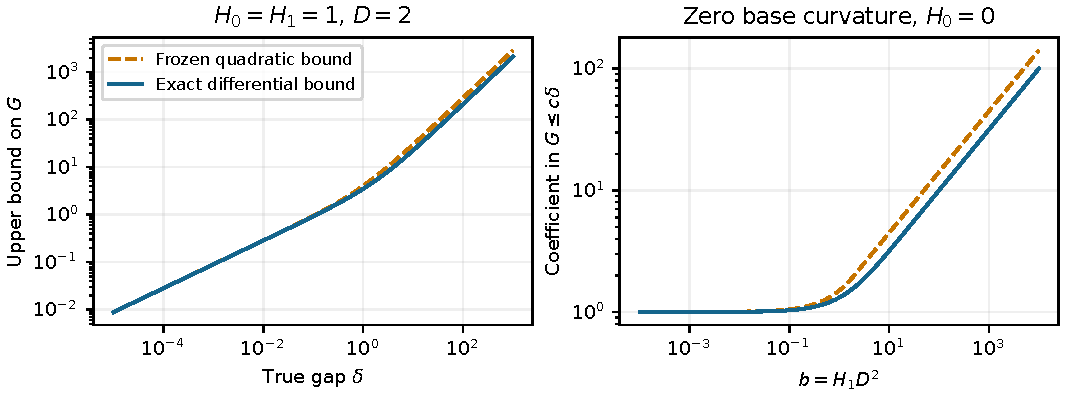
\includegraphics[width=\linewidth]{figures/gap_geometry.pdf}
\caption{Pointwise theoretical bounds. The differential envelope retains
the changing function value along the segment; the frozen quadratic
comparison is~\eqref{eq:sharpbridge}. At zero base curvature, the exact
linear coefficient is $\sqrt b\coth\sqrt b$. These are inequalities
over a function class, not optimization trajectories or timing results.}
\label{fig:geometry}
\end{figure}

\begin{theorem}[Geometric AFW certificate bound]\label{thm:geometric}
Assume $H_0+H_1>0$ and~\eqref{eq:geometry}. Set
\[
 J_*=\ceil{\log_2(U_0/\eta_\varepsilon)},\qquad
 P_*=\ceil{\log_2\max\{1,M/[2(H_0+H_1U_0)]\}}.
\]
For $0<\varepsilon<U_0$, the same algorithm reaches
$U_N\le\varepsilon$ within
\begin{equation}\label{eq:geometriccount}
 N\le2\ceil{P_*+(6+4H_0D^2/\kappa)J_*+8H_1D^2U_0/\kappa}
       +|S_0|-1.
\end{equation}
Equation~\eqref{eq:functioncount} remains valid. None of
$H_0,H_1,\kappa,f_Q^*$ is an algorithm input.
\end{theorem}
\begin{proof}
Analyze true-error phases $b_j/2<\delta_k\le b_j$ with
$b_j=U_0/2^j$, until $\delta\le\eta_\varepsilon$.
Their positive caps $C_j=2(H_0+H_1b_j)$ decrease by at most a factor
two. The initial true error may skip phases; Lemma~\ref{lem:lag}
still bounds lag updates by $P_*+J_*$.
On a controlled good step,
\[
 f_k-f_{k+1}\ge\delta_k\min\{1/2,\kappa/(C_jD^2)\}
 >\min\{b_j/4,\kappa b_j/(2C_jD^2)\}.
\]
For a full FW step use $g\ge G\ge\delta$; for a nonclipped step
use~\eqref{eq:geometry}. The phase budget $b_j$ permits at most
$5+4H_0D^2/\kappa+4H_1D^2b_j/\kappa$ controlled good updates.
Sum $\sum_{j<J_*}b_j<2U_0$, add lag updates and
apply~\eqref{eq:dropcount}. Theorem~\ref{lem:bridge} ensures the actual
certificate has passed by this point.
\end{proof}

For fixed problem and initialization the accuracy dependence is
logarithmic. The explicit $H_1$ phase cost is proportional to $U_0$;
$H_1$ also enters $J_*$ through~\eqref{eq:threshold}.
Both AFW bounds apply when the geometric hypothesis holds; the
initial $U_0/\kappa$ contribution means the geometric bound is not
uniformly tighter than the convex one.
One need not assume $H_0>0$: the caps are positive at positive phase
levels when $H_1>0$. A nonaffine example is $f=t+(\max\{t,0\})^3$,
$t=1/2-x$, on $[-1/2,1/2]$, with $H_0=0,H_1=6$ and
$\kappa=1/16$ (Appendix~\ref{app:bridge}). In fact $H_0=0$ has
stronger structural consequences, proved next without assuming
the geometric inequality~\eqref{eq:geometry}.
